\documentclass[1p]{elsarticle_modified}
%\bibliographystyle{elsarticle-num}

%\usepackage[colorlinks]{hyperref}
%\usepackage{abbrmath_seonhwa} %\Abb, \Ascr, \Acal ,\Abf, \Afrak
\usepackage{amsfonts}
\usepackage{amssymb}
\usepackage{amsmath}
\usepackage{amsthm}
\usepackage{scalefnt}
\usepackage{amsbsy}
\usepackage{kotex}
\usepackage{caption}
\usepackage{subfig}
\usepackage{color}
\usepackage{graphicx}
\usepackage{xcolor} %% white, black, red, green, blue, cyan, magenta, yellow
\usepackage{float}
\usepackage{setspace}
\usepackage{hyperref}

\usepackage{tikz}
\usetikzlibrary{arrows}

\usepackage{multirow}
\usepackage{array} % fixed length table
\usepackage{hhline}

%%%%%%%%%%%%%%%%%%%%%
\makeatletter
\renewcommand*\env@matrix[1][\arraystretch]{%
	\edef\arraystretch{#1}%
	\hskip -\arraycolsep
	\let\@ifnextchar\new@ifnextchar
	\array{*\c@MaxMatrixCols c}}
\makeatother %https://tex.stackexchange.com/questions/14071/how-can-i-increase-the-line-spacing-in-a-matrix
%%%%%%%%%%%%%%%

\usepackage[normalem]{ulem}

\newcommand{\msout}[1]{\ifmmode\text{\sout{\ensuremath{#1}}}\else\sout{#1}\fi}
%SOURCE: \msout is \stkout macro in https://tex.stackexchange.com/questions/20609/strikeout-in-math-mode

\newcommand{\cancel}[1]{
	\ifmmode
	{\color{red}\msout{#1}}
	\else
	{\color{red}\sout{#1}}
	\fi
}

\newcommand{\add}[1]{
	{\color{blue}\uwave{#1}}
}

\newcommand{\replace}[2]{
	\ifmmode
	{\color{red}\msout{#1}}{\color{blue}\uwave{#2}}
	\else
	{\color{red}\sout{#1}}{\color{blue}\uwave{#2}}
	\fi
}

\newcommand{\Sol}{\mathcal{S}} %segment
\newcommand{\D}{D} %diagram
\newcommand{\A}{\mathcal{A}} %arc


%%%%%%%%%%%%%%%%%%%%%%%%%%%%%5 test

\def\sl{\operatorname{\textup{SL}}(2,\Cbb)}
\def\psl{\operatorname{\textup{PSL}}(2,\Cbb)}
\def\quan{\mkern 1mu \triangleright \mkern 1mu}

\theoremstyle{definition}
\newtheorem{thm}{Theorem}[section]
\newtheorem{prop}[thm]{Proposition}
\newtheorem{lem}[thm]{Lemma}
\newtheorem{ques}[thm]{Question}
\newtheorem{cor}[thm]{Corollary}
\newtheorem{defn}[thm]{Definition}
\newtheorem{exam}[thm]{Example}
\newtheorem{rmk}[thm]{Remark}
\newtheorem{alg}[thm]{Algorithm}

\newcommand{\I}{\sqrt{-1}}
\begin{document}

%\begin{frontmatter}
%
%\title{Boundary parabolic representations of knots up to 8 crossings}
%
%%% Group authors per affiliation:
%\author{Yunhi Cho} 
%\address{Department of Mathematics, University of Seoul, Seoul, Korea}
%\ead{yhcho@uos.ac.kr}
%
%
%\author{Seonhwa Kim} %\fnref{s_kim}}
%\address{Center for Geometry and Physics, Institute for Basic Science, Pohang, 37673, Korea}
%\ead{ryeona17@ibs.re.kr}
%
%\author{Hyuk Kim}
%\address{Department of Mathematical Sciences, Seoul National University, Seoul 08826, Korea}
%\ead{hyukkim@snu.ac.kr}
%
%\author{Seokbeom Yoon}
%\address{Department of Mathematical Sciences, Seoul National University, Seoul, 08826,  Korea}
%\ead{sbyoon15@snu.ac.kr}
%
%\begin{abstract}
%We find all boundary parabolic representation of knots up to 8 crossings.
%
%\end{abstract}
%\begin{keyword}
%    \MSC[2010] 57M25 
%\end{keyword}
%
%\end{frontmatter}

%\linenumbers
%\tableofcontents
%
\newcommand\colored[1]{\textcolor{white}{\rule[-0.35ex]{0.8em}{1.4ex}}\kern-0.8em\color{red} #1}%
%\newcommand\colored[1]{\textcolor{white}{ #1}\kern-2.17ex	\textcolor{white}{ #1}\kern-1.81ex	\textcolor{white}{ #1}\kern-2.15ex\color{red}#1	}

{\Large $\underline{11a_{152}~(K11a_{152})}$}

\setlength{\tabcolsep}{10pt}
\renewcommand{\arraystretch}{1.6}
\vspace{1cm}\begin{tabular}{m{100pt}>{\centering\arraybackslash}m{274pt}}
\multirow{5}{120pt}{
	\centering
	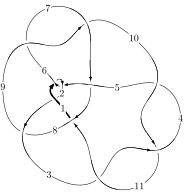
\includegraphics[width=112pt]{../../../GIT/diagram.site/Diagrams/png/401_11a_152.png}\\
\ \ \ A knot diagram\footnotemark}&
\allowdisplaybreaks
\textbf{Linearized knot diagam} \\
\cline{2-2}
 &
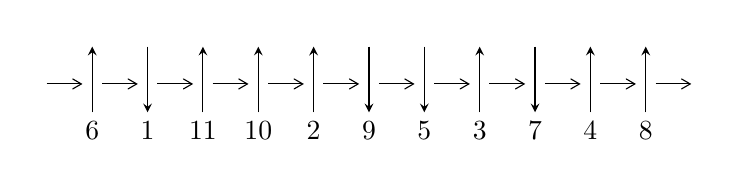
\begin{tikzpicture}[x=20pt, y=17pt]
	% nodes
	\node (C0) at (0, 0) {};
	\node (C1) at (1, 0) {};
	\node (C1U) at (1, +1) {};
	\node (C1D) at (1, -1) {6};

	\node (C2) at (2, 0) {};
	\node (C2U) at (2, +1) {};
	\node (C2D) at (2, -1) {1};

	\node (C3) at (3, 0) {};
	\node (C3U) at (3, +1) {};
	\node (C3D) at (3, -1) {11};

	\node (C4) at (4, 0) {};
	\node (C4U) at (4, +1) {};
	\node (C4D) at (4, -1) {10};

	\node (C5) at (5, 0) {};
	\node (C5U) at (5, +1) {};
	\node (C5D) at (5, -1) {2};

	\node (C6) at (6, 0) {};
	\node (C6U) at (6, +1) {};
	\node (C6D) at (6, -1) {9};

	\node (C7) at (7, 0) {};
	\node (C7U) at (7, +1) {};
	\node (C7D) at (7, -1) {5};

	\node (C8) at (8, 0) {};
	\node (C8U) at (8, +1) {};
	\node (C8D) at (8, -1) {3};

	\node (C9) at (9, 0) {};
	\node (C9U) at (9, +1) {};
	\node (C9D) at (9, -1) {7};

	\node (C10) at (10, 0) {};
	\node (C10U) at (10, +1) {};
	\node (C10D) at (10, -1) {4};

	\node (C11) at (11, 0) {};
	\node (C11U) at (11, +1) {};
	\node (C11D) at (11, -1) {8};
	\node (C12) at (12, 0) {};

	% arrows
	\draw[->,>={angle 60}]
	(C0) edge (C1) (C1) edge (C2) (C2) edge (C3) (C3) edge (C4) (C4) edge (C5) (C5) edge (C6) (C6) edge (C7) (C7) edge (C8) (C8) edge (C9) (C9) edge (C10) (C10) edge (C11) (C11) edge (C12) ;	\draw[->,>=stealth]
	(C1D) edge (C1U) (C2U) edge (C2D) (C3D) edge (C3U) (C4D) edge (C4U) (C5D) edge (C5U) (C6U) edge (C6D) (C7U) edge (C7D) (C8D) edge (C8U) (C9U) edge (C9D) (C10D) edge (C10U) (C11D) edge (C11U) ;
	\end{tikzpicture} \\
\hhline{~~} \\& 
\textbf{Solving Sequence} \\ \cline{2-2} 
 &
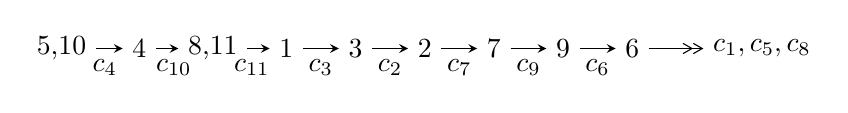
\begin{tikzpicture}[x=25pt, y=7pt]
	% node
	\node (A0) at (-1/8, 0) {5,10};
	\node (A1) at (1, 0) {4};
	\node (A2) at (33/16, 0) {8,11};
	\node (A3) at (25/8, 0) {1};
	\node (A4) at (33/8, 0) {3};
	\node (A5) at (41/8, 0) {2};
	\node (A6) at (49/8, 0) {7};
	\node (A7) at (57/8, 0) {9};
	\node (A8) at (65/8, 0) {6};
	\node (C1) at (1/2, -1) {$c_{4}$};
	\node (C2) at (3/2, -1) {$c_{10}$};
	\node (C3) at (21/8, -1) {$c_{11}$};
	\node (C4) at (29/8, -1) {$c_{3}$};
	\node (C5) at (37/8, -1) {$c_{2}$};
	\node (C6) at (45/8, -1) {$c_{7}$};
	\node (C7) at (53/8, -1) {$c_{9}$};
	\node (C8) at (61/8, -1) {$c_{6}$};
	\node (A9) at (10, 0) {$c_{1},c_{5},c_{8}$};

	% edge
	\draw[->,>=stealth]	
	(A0) edge (A1) (A1) edge (A2) (A2) edge (A3) (A3) edge (A4) (A4) edge (A5) (A5) edge (A6) (A6) edge (A7) (A7) edge (A8) ;
	\draw[->>,>={angle 60}]	
	(A8) edge (A9);
\end{tikzpicture} \\ 

\end{tabular} \\

\footnotetext{
The image of knot diagram is generated by the software ``\textbf{Draw programme}" developed by Andrew Bartholomew(\url{http://www.layer8.co.uk/maths/draw/index.htm\#Running-draw}), where we modified some parts for our purpose(\url{https://github.com/CATsTAILs/LinksPainter}).
}\phantom \\ \newline 
\centering \textbf{Ideals for irreducible components\footnotemark of $X_{\text{par}}$} 
 
\begin{align*}
I^u_{1}&=\langle 
3.06173\times10^{60} u^{58}-4.84579\times10^{60} u^{57}+\cdots+7.53869\times10^{60} b-6.50731\times10^{60},\\
\phantom{I^u_{1}}&\phantom{= \langle  }3.66584\times10^{60} u^{58}-7.89631\times10^{60} u^{57}+\cdots+7.53869\times10^{60} a-4.93339\times10^{60},\;u^{59}-2 u^{58}+\cdots-2 u+1\rangle \\
I^u_{2}&=\langle 
3 b-2,\;3 a-1,\;u-1\rangle \\
\\
\end{align*}
\raggedright * 2 irreducible components of $\dim_{\mathbb{C}}=0$, with total 60 representations.\\
\footnotetext{All coefficients of polynomials are rational numbers. But the coefficients are sometimes approximated in decimal forms when there is not enough margin.}
\newpage
\renewcommand{\arraystretch}{1}
\centering \section*{I. $I^u_{1}= \langle 3.06\times10^{60} u^{58}-4.85\times10^{60} u^{57}+\cdots+7.54\times10^{60} b-6.51\times10^{60},\;3.67\times10^{60} u^{58}-7.90\times10^{60} u^{57}+\cdots+7.54\times10^{60} a-4.93\times10^{60},\;u^{59}-2 u^{58}+\cdots-2 u+1 \rangle$}
\flushleft \textbf{(i) Arc colorings}\\
\begin{tabular}{m{7pt} m{180pt} m{7pt} m{180pt} }
\flushright $a_{5}=$&$\begin{pmatrix}1\\0\end{pmatrix}$ \\
\flushright $a_{10}=$&$\begin{pmatrix}0\\u\end{pmatrix}$ \\
\flushright $a_{4}=$&$\begin{pmatrix}1\\u^2\end{pmatrix}$ \\
\flushright $a_{8}=$&$\begin{pmatrix}-0.486270 u^{58}+1.04744 u^{57}+\cdots-3.97604 u+0.654410\\-0.406136 u^{58}+0.642788 u^{57}+\cdots+0.0112412 u+0.863189\end{pmatrix}$ \\
\flushright $a_{11}=$&$\begin{pmatrix}u\\u^3+u\end{pmatrix}$ \\
\flushright $a_{1}=$&$\begin{pmatrix}0.162396 u^{58}-0.0414876 u^{57}+\cdots-0.620453 u+0.289562\\0.264365 u^{58}-0.566519 u^{57}+\cdots-0.385454 u-0.631376\end{pmatrix}$ \\
\flushright $a_{3}=$&$\begin{pmatrix}u^2+1\\u^4+2 u^2\end{pmatrix}$ \\
\flushright $a_{2}=$&$\begin{pmatrix}-0.418108 u^{58}+0.310255 u^{57}+\cdots-0.686190 u+0.663142\\-0.104972 u^{58}+0.436443 u^{57}+\cdots-0.736202 u+0.995922\end{pmatrix}$ \\
\flushright $a_{7}=$&$\begin{pmatrix}-0.892406 u^{58}+1.69023 u^{57}+\cdots-3.96480 u+1.51760\\-0.406136 u^{58}+0.642788 u^{57}+\cdots+0.0112412 u+0.863189\end{pmatrix}$ \\
\flushright $a_{9}=$&$\begin{pmatrix}-0.855262 u^{58}+1.72021 u^{57}+\cdots-3.82594 u+1.72628\\-0.432378 u^{58}+0.672814 u^{57}+\cdots+1.00305 u+0.933233\end{pmatrix}$ \\
\flushright $a_{6}=$&$\begin{pmatrix}-0.0187345 u^{58}-0.208269 u^{57}+\cdots-0.169215 u-0.637633\\-0.0593368 u^{58}+0.0928833 u^{57}+\cdots-1.26241 u-0.102333\end{pmatrix}$\\ \flushright $a_{6}=$&$\begin{pmatrix}-0.0187345 u^{58}-0.208269 u^{57}+\cdots-0.169215 u-0.637633\\-0.0593368 u^{58}+0.0928833 u^{57}+\cdots-1.26241 u-0.102333\end{pmatrix}$\\&\end{tabular}
\flushleft \textbf{(ii) Obstruction class $= -1$}\\~\\
\flushleft \textbf{(iii) Cusp Shapes $= 0.834501 u^{58}-3.42749 u^{57}+\cdots-17.5070 u-8.87218$}\\~\\
\newpage\renewcommand{\arraystretch}{1}
\flushleft \textbf{(iv) u-Polynomials at the component}\newline \\
\begin{tabular}{m{50pt}|m{274pt}}
Crossings & \hspace{64pt}u-Polynomials at each crossing \\
\hline $$\begin{aligned}c_{1},c_{5}\end{aligned}$$&$\begin{aligned}
&u^{59}-2 u^{58}+\cdots+2 u-1
\end{aligned}$\\
\hline $$\begin{aligned}c_{2}\end{aligned}$$&$\begin{aligned}
&u^{59}+24 u^{58}+\cdots-4 u-1
\end{aligned}$\\
\hline $$\begin{aligned}c_{3},c_{4},c_{10}\end{aligned}$$&$\begin{aligned}
&u^{59}+2 u^{58}+\cdots-2 u-1
\end{aligned}$\\
\hline $$\begin{aligned}c_{6},c_{9}\end{aligned}$$&$\begin{aligned}
&u^{59}-2 u^{58}+\cdots-32 u-9
\end{aligned}$\\
\hline $$\begin{aligned}c_{7}\end{aligned}$$&$\begin{aligned}
&3(3 u^{59}+29 u^{58}+\cdots+96336 u-7216)
\end{aligned}$\\
\hline $$\begin{aligned}c_{8}\end{aligned}$$&$\begin{aligned}
&3(3 u^{59}-44 u^{58}+\cdots-96 u-64)
\end{aligned}$\\
\hline $$\begin{aligned}c_{11}\end{aligned}$$&$\begin{aligned}
&u^{59}-5 u^{58}+\cdots+108 u-18
\end{aligned}$\\
\hline
\end{tabular}\\~\\
\newpage\renewcommand{\arraystretch}{1}
\flushleft \textbf{(v) Riley Polynomials at the component}\newline \\
\begin{tabular}{m{50pt}|m{274pt}}
Crossings & \hspace{64pt}Riley Polynomials at each crossing \\
\hline $$\begin{aligned}c_{1},c_{5}\end{aligned}$$&$\begin{aligned}
&y^{59}+24 y^{58}+\cdots-4 y-1
\end{aligned}$\\
\hline $$\begin{aligned}c_{2}\end{aligned}$$&$\begin{aligned}
&y^{59}+16 y^{58}+\cdots-76 y-1
\end{aligned}$\\
\hline $$\begin{aligned}c_{3},c_{4},c_{10}\end{aligned}$$&$\begin{aligned}
&y^{59}+60 y^{58}+\cdots-4 y-1
\end{aligned}$\\
\hline $$\begin{aligned}c_{6},c_{9}\end{aligned}$$&$\begin{aligned}
&y^{59}-44 y^{58}+\cdots+3472 y-81
\end{aligned}$\\
\hline $$\begin{aligned}c_{7}\end{aligned}$$&$\begin{aligned}
&9(9 y^{59}-787 y^{58}+\cdots+4.57874\times10^{9} y-5.20707\times10^{7})
\end{aligned}$\\
\hline $$\begin{aligned}c_{8}\end{aligned}$$&$\begin{aligned}
&9(9 y^{59}-424 y^{58}+\cdots-148480 y-4096)
\end{aligned}$\\
\hline $$\begin{aligned}c_{11}\end{aligned}$$&$\begin{aligned}
&y^{59}+9 y^{58}+\cdots-6300 y-324
\end{aligned}$\\
\hline
\end{tabular}\\~\\
\newpage\flushleft \textbf{(vi) Complex Volumes and Cusp Shapes}
$$\begin{array}{c|c|c}  
\text{Solutions to }I^u_{1}& \I (\text{vol} + \sqrt{-1}CS) & \text{Cusp shape}\\
 \hline 
\begin{aligned}
u &= \phantom{-}0.772835 + 0.630169 I \\
a &= \phantom{-}0.486457 + 0.408560 I \\
b &= -1.20441 + 0.80693 I\end{aligned}
 & -2.98475 + 11.82370 I & \phantom{-0.000000 } 0. - 9.15160 I \\ \hline\begin{aligned}
u &= \phantom{-}0.772835 - 0.630169 I \\
a &= \phantom{-}0.486457 - 0.408560 I \\
b &= -1.20441 - 0.80693 I\end{aligned}
 & -2.98475 - 11.82370 I & \phantom{-0.000000 -}0. + 9.15160 I \\ \hline\begin{aligned}
u &= \phantom{-}0.893809 + 0.462202 I \\
a &= -0.354680 + 0.593555 I \\
b &= -0.839382 - 0.317177 I\end{aligned}
 & -2.42227 - 6.38133 I & \phantom{-0.000000 } 0 \\ \hline\begin{aligned}
u &= \phantom{-}0.893809 - 0.462202 I \\
a &= -0.354680 - 0.593555 I \\
b &= -0.839382 + 0.317177 I\end{aligned}
 & -2.42227 + 6.38133 I & \phantom{-0.000000 } 0 \\ \hline\begin{aligned}
u &= -0.769320 + 0.665358 I \\
a &= -0.399111 + 0.329878 I \\
b &= \phantom{-}1.017530 + 0.758404 I\end{aligned}
 & -0.73398 - 6.05254 I & \phantom{-0.000000 } 0 \\ \hline\begin{aligned}
u &= -0.769320 - 0.665358 I \\
a &= -0.399111 - 0.329878 I \\
b &= \phantom{-}1.017530 - 0.758404 I\end{aligned}
 & -0.73398 + 6.05254 I & \phantom{-0.000000 } 0 \\ \hline\begin{aligned}
u &= \phantom{-}0.871014 + 0.643445 I \\
a &= \phantom{-}0.171049 + 0.483786 I \\
b &= -1.045410 + 0.327693 I\end{aligned}
 & -7.08101 + 2.98588 I & \phantom{-0.000000 } 0 \\ \hline\begin{aligned}
u &= \phantom{-}0.871014 - 0.643445 I \\
a &= \phantom{-}0.171049 - 0.483786 I \\
b &= -1.045410 - 0.327693 I\end{aligned}
 & -7.08101 - 2.98588 I & \phantom{-0.000000 } 0 \\ \hline\begin{aligned}
u &= -1.058830 + 0.406799 I \\
a &= \phantom{-}0.273276 + 0.303483 I \\
b &= \phantom{-}0.621331 - 0.083380 I\end{aligned}
 & \phantom{-}0.196305 + 0.379080 I & \phantom{-0.000000 } 0 \\ \hline\begin{aligned}
u &= -1.058830 - 0.406799 I \\
a &= \phantom{-}0.273276 - 0.303483 I \\
b &= \phantom{-}0.621331 + 0.083380 I\end{aligned}
 & \phantom{-}0.196305 - 0.379080 I & \phantom{-0.000000 } 0\\
 \hline 
 \end{array}$$\newpage$$\begin{array}{c|c|c}  
\text{Solutions to }I^u_{1}& \I (\text{vol} + \sqrt{-1}CS) & \text{Cusp shape}\\
 \hline 
\begin{aligned}
u &= -0.421425 + 0.652253 I \\
a &= -0.229200 - 0.191547 I \\
b &= \phantom{-}0.073389 + 0.936603 I\end{aligned}
 & \phantom{-}1.67726 - 2.08783 I & \phantom{-}6.30981 + 5.41216 I \\ \hline\begin{aligned}
u &= -0.421425 - 0.652253 I \\
a &= -0.229200 + 0.191547 I \\
b &= \phantom{-}0.073389 - 0.936603 I\end{aligned}
 & \phantom{-}1.67726 + 2.08783 I & \phantom{-}6.30981 - 5.41216 I \\ \hline\begin{aligned}
u &= \phantom{-}0.538558 + 0.434252 I \\
a &= -1.52889 - 0.28560 I \\
b &= \phantom{-}0.560561 - 0.856660 I\end{aligned}
 & \phantom{-}1.09865 + 6.46666 I & \phantom{-}3.55713 - 8.78536 I \\ \hline\begin{aligned}
u &= \phantom{-}0.538558 - 0.434252 I \\
a &= -1.52889 + 0.28560 I \\
b &= \phantom{-}0.560561 + 0.856660 I\end{aligned}
 & \phantom{-}1.09865 - 6.46666 I & \phantom{-}3.55713 + 8.78536 I \\ \hline\begin{aligned}
u &= -0.564831 + 0.382666 I \\
a &= \phantom{-}1.263980 - 0.143409 I \\
b &= -0.352394 - 0.726889 I\end{aligned}
 & \phantom{-}2.45484 - 1.46486 I & \phantom{-}7.14865 + 3.00711 I \\ \hline\begin{aligned}
u &= -0.564831 - 0.382666 I \\
a &= \phantom{-}1.263980 + 0.143409 I \\
b &= -0.352394 + 0.726889 I\end{aligned}
 & \phantom{-}2.45484 + 1.46486 I & \phantom{-}7.14865 - 3.00711 I \\ \hline\begin{aligned}
u &= \phantom{-}0.407938 + 0.495194 I \\
a &= \phantom{-}0.234399 - 0.376842 I \\
b &= \phantom{-}0.290086 + 1.044180 I\end{aligned}
 & \phantom{-}0.82881 - 3.06030 I & \phantom{-}4.18689 + 0.59937 I \\ \hline\begin{aligned}
u &= \phantom{-}0.407938 - 0.495194 I \\
a &= \phantom{-}0.234399 + 0.376842 I \\
b &= \phantom{-}0.290086 - 1.044180 I\end{aligned}
 & \phantom{-}0.82881 + 3.06030 I & \phantom{-}4.18689 - 0.59937 I \\ \hline\begin{aligned}
u &= -0.133674 + 1.400600 I \\
a &= \phantom{-}1.029390 - 0.297689 I \\
b &= -0.654687 + 0.290826 I\end{aligned}
 & -3.80970 - 2.30389 I & \phantom{-0.000000 } 0 \\ \hline\begin{aligned}
u &= -0.133674 - 1.400600 I \\
a &= \phantom{-}1.029390 + 0.297689 I \\
b &= -0.654687 - 0.290826 I\end{aligned}
 & -3.80970 + 2.30389 I & \phantom{-0.000000 } 0\\
 \hline 
 \end{array}$$\newpage$$\begin{array}{c|c|c}  
\text{Solutions to }I^u_{1}& \I (\text{vol} + \sqrt{-1}CS) & \text{Cusp shape}\\
 \hline 
\begin{aligned}
u &= \phantom{-}0.065188 + 1.410510 I \\
a &= -0.86471 - 1.34195 I \\
b &= \phantom{-}0.80222 + 1.22589 I\end{aligned}
 & -5.12435 - 1.84537 I & \phantom{-0.000000 } 0 \\ \hline\begin{aligned}
u &= \phantom{-}0.065188 - 1.410510 I \\
a &= -0.86471 + 1.34195 I \\
b &= \phantom{-}0.80222 - 1.22589 I\end{aligned}
 & -5.12435 + 1.84537 I & \phantom{-0.000000 } 0 \\ \hline\begin{aligned}
u &= -0.240543 + 0.535915 I \\
a &= \phantom{-}1.08834 - 2.33107 I \\
b &= -1.011390 + 0.003314 I\end{aligned}
 & -3.33182 - 4.55345 I & -4.30626 + 8.52736 I \\ \hline\begin{aligned}
u &= -0.240543 - 0.535915 I \\
a &= \phantom{-}1.08834 + 2.33107 I \\
b &= -1.011390 - 0.003314 I\end{aligned}
 & -3.33182 + 4.55345 I & -4.30626 - 8.52736 I \\ \hline\begin{aligned}
u &= \phantom{-}0.01950 + 1.43251 I \\
a &= -6.58810 + 3.57964 I \\
b &= \phantom{-}6.56362 - 4.27440 I\end{aligned}
 & -6.55441 + 2.12552 I & \phantom{-0.000000 } 0 \\ \hline\begin{aligned}
u &= \phantom{-}0.01950 - 1.43251 I \\
a &= -6.58810 - 3.57964 I \\
b &= \phantom{-}6.56362 + 4.27440 I\end{aligned}
 & -6.55441 - 2.12552 I & \phantom{-0.000000 } 0 \\ \hline\begin{aligned}
u &= -0.087504 + 0.546858 I \\
a &= \phantom{-}0.39073 - 2.81411 I \\
b &= -0.423741 + 0.227336 I\end{aligned}
 & -4.10264 + 1.33087 I & -6.62416 - 1.43922 I \\ \hline\begin{aligned}
u &= -0.087504 - 0.546858 I \\
a &= \phantom{-}0.39073 + 2.81411 I \\
b &= -0.423741 - 0.227336 I\end{aligned}
 & -4.10264 - 1.33087 I & -6.62416 + 1.43922 I \\ \hline\begin{aligned}
u &= -0.541912\phantom{ +0.000000I} \\
a &= \phantom{-}0.611273\phantom{ +0.000000I} \\
b &= -0.123892\phantom{ +0.000000I}\end{aligned}
 & \phantom{-}0.892681\phantom{ +0.000000I} & \phantom{-}11.5980\phantom{ +0.000000I} \\ \hline\begin{aligned}
u &= \phantom{-}0.356131 + 0.401711 I \\
a &= -0.91403 - 1.19911 I \\
b &= \phantom{-}0.886772 - 0.315941 I\end{aligned}
 & -1.79094 + 1.03849 I & -2.00439 - 5.37844 I\\
 \hline 
 \end{array}$$\newpage$$\begin{array}{c|c|c}  
\text{Solutions to }I^u_{1}& \I (\text{vol} + \sqrt{-1}CS) & \text{Cusp shape}\\
 \hline 
\begin{aligned}
u &= \phantom{-}0.356131 - 0.401711 I \\
a &= -0.91403 + 1.19911 I \\
b &= \phantom{-}0.886772 + 0.315941 I\end{aligned}
 & -1.79094 - 1.03849 I & -2.00439 + 5.37844 I \\ \hline\begin{aligned}
u &= -0.15816 + 1.47252 I \\
a &= \phantom{-}1.59643 + 0.26788 I \\
b &= -0.817080 - 0.366010 I\end{aligned}
 & -3.60110 - 3.99693 I & \phantom{-0.000000 } 0 \\ \hline\begin{aligned}
u &= -0.15816 - 1.47252 I \\
a &= \phantom{-}1.59643 - 0.26788 I \\
b &= -0.817080 + 0.366010 I\end{aligned}
 & -3.60110 + 3.99693 I & \phantom{-0.000000 } 0 \\ \hline\begin{aligned}
u &= \phantom{-}0.10761 + 1.48343 I \\
a &= -1.90601 - 0.15341 I \\
b &= \phantom{-}1.253580 - 0.326367 I\end{aligned}
 & -7.99699 + 2.70852 I & \phantom{-0.000000 } 0 \\ \hline\begin{aligned}
u &= \phantom{-}0.10761 - 1.48343 I \\
a &= -1.90601 + 0.15341 I \\
b &= \phantom{-}1.253580 + 0.326367 I\end{aligned}
 & -7.99699 - 2.70852 I & \phantom{-0.000000 } 0 \\ \hline\begin{aligned}
u &= \phantom{-}0.04741 + 1.49720 I \\
a &= -1.53150 - 0.05275 I \\
b &= \phantom{-}1.18789 - 0.84677 I\end{aligned}
 & -8.07186 + 1.71448 I & \phantom{-0.000000 } 0 \\ \hline\begin{aligned}
u &= \phantom{-}0.04741 - 1.49720 I \\
a &= -1.53150 + 0.05275 I \\
b &= \phantom{-}1.18789 + 0.84677 I\end{aligned}
 & -8.07186 - 1.71448 I & \phantom{-0.000000 } 0 \\ \hline\begin{aligned}
u &= \phantom{-}0.15594 + 1.49285 I \\
a &= -1.83827 + 0.36366 I \\
b &= \phantom{-}0.915367 - 0.530137 I\end{aligned}
 & -5.23405 + 8.92854 I & \phantom{-0.000000 } 0 \\ \hline\begin{aligned}
u &= \phantom{-}0.15594 - 1.49285 I \\
a &= -1.83827 - 0.36366 I \\
b &= \phantom{-}0.915367 + 0.530137 I\end{aligned}
 & -5.23405 - 8.92854 I & \phantom{-0.000000 } 0 \\ \hline\begin{aligned}
u &= -0.05816 + 1.52227 I \\
a &= \phantom{-}1.62424 - 0.57913 I \\
b &= -1.082160 - 0.473836 I\end{aligned}
 & -10.18440 - 5.57197 I & \phantom{-0.000000 } 0\\
 \hline 
 \end{array}$$\newpage$$\begin{array}{c|c|c}  
\text{Solutions to }I^u_{1}& \I (\text{vol} + \sqrt{-1}CS) & \text{Cusp shape}\\
 \hline 
\begin{aligned}
u &= -0.05816 - 1.52227 I \\
a &= \phantom{-}1.62424 + 0.57913 I \\
b &= -1.082160 + 0.473836 I\end{aligned}
 & -10.18440 + 5.57197 I & \phantom{-0.000000 } 0 \\ \hline\begin{aligned}
u &= -0.02356 + 1.52322 I \\
a &= \phantom{-}0.755412 - 0.573027 I \\
b &= -0.529705 - 0.615962 I\end{aligned}
 & -10.99430 + 0.93911 I & \phantom{-0.000000 } 0 \\ \hline\begin{aligned}
u &= -0.02356 - 1.52322 I \\
a &= \phantom{-}0.755412 + 0.573027 I \\
b &= -0.529705 + 0.615962 I\end{aligned}
 & -10.99430 - 0.93911 I & \phantom{-0.000000 } 0 \\ \hline\begin{aligned}
u &= \phantom{-}0.226157 + 0.399881 I \\
a &= -0.44978 - 1.85794 I \\
b &= \phantom{-}0.880240 - 0.289353 I\end{aligned}
 & -1.71907 + 0.84714 I & -1.58416 - 2.44825 I \\ \hline\begin{aligned}
u &= \phantom{-}0.226157 - 0.399881 I \\
a &= -0.44978 + 1.85794 I \\
b &= \phantom{-}0.880240 + 0.289353 I\end{aligned}
 & -1.71907 - 0.84714 I & -1.58416 + 2.44825 I \\ \hline\begin{aligned}
u &= \phantom{-}0.338130 + 0.233977 I \\
a &= \phantom{-}0.284402 - 0.906149 I \\
b &= \phantom{-}1.53304 + 0.15644 I\end{aligned}
 & -1.34852 + 1.21434 I & -0.61490 - 9.36280 I \\ \hline\begin{aligned}
u &= \phantom{-}0.338130 - 0.233977 I \\
a &= \phantom{-}0.284402 + 0.906149 I \\
b &= \phantom{-}1.53304 - 0.15644 I\end{aligned}
 & -1.34852 - 1.21434 I & -0.61490 + 9.36280 I \\ \hline\begin{aligned}
u &= \phantom{-}0.25843 + 1.57442 I \\
a &= \phantom{-}1.86661 - 0.09363 I \\
b &= -1.66038 + 1.05895 I\end{aligned}
 & -10.2296 + 15.6414 I & \phantom{-0.000000 } 0 \\ \hline\begin{aligned}
u &= \phantom{-}0.25843 - 1.57442 I \\
a &= \phantom{-}1.86661 + 0.09363 I \\
b &= -1.66038 - 1.05895 I\end{aligned}
 & -10.2296 - 15.6414 I & \phantom{-0.000000 } 0 \\ \hline\begin{aligned}
u &= -0.25542 + 1.58255 I \\
a &= -1.69347 - 0.15977 I \\
b &= \phantom{-}1.51201 + 1.06731 I\end{aligned}
 & -8.11873 - 9.85959 I & \phantom{-0.000000 } 0\\
 \hline 
 \end{array}$$\newpage$$\begin{array}{c|c|c}  
\text{Solutions to }I^u_{1}& \I (\text{vol} + \sqrt{-1}CS) & \text{Cusp shape}\\
 \hline 
\begin{aligned}
u &= -0.25542 - 1.58255 I \\
a &= -1.69347 + 0.15977 I \\
b &= \phantom{-}1.51201 - 1.06731 I\end{aligned}
 & -8.11873 + 9.85959 I & \phantom{-0.000000 } 0 \\ \hline\begin{aligned}
u &= \phantom{-}0.27503 + 1.58999 I \\
a &= \phantom{-}1.46114 + 0.16066 I \\
b &= -1.41360 + 0.76345 I\end{aligned}
 & -14.4364 + 7.1649 I & \phantom{-0.000000 } 0 \\ \hline\begin{aligned}
u &= \phantom{-}0.27503 - 1.58999 I \\
a &= \phantom{-}1.46114 - 0.16066 I \\
b &= -1.41360 - 0.76345 I\end{aligned}
 & -14.4364 - 7.1649 I & \phantom{-0.000000 } 0 \\ \hline\begin{aligned}
u &= -0.359471 + 0.100084 I \\
a &= -0.622900 - 0.492336 I \\
b &= -2.26496 + 0.09975 I\end{aligned}
 & -2.01075 + 2.52108 I & \phantom{-}10.02369 + 7.46616 I \\ \hline\begin{aligned}
u &= -0.359471 - 0.100084 I \\
a &= -0.622900 + 0.492336 I \\
b &= -2.26496 - 0.09975 I\end{aligned}
 & -2.01075 - 2.52108 I & \phantom{-}10.02369 - 7.46616 I \\ \hline\begin{aligned}
u &= \phantom{-}0.34658 + 1.62518 I \\
a &= \phantom{-}0.678378 + 0.241908 I \\
b &= -0.828238 + 0.485899 I\end{aligned}
 & -9.14972 - 1.51752 I & \phantom{-0.000000 } 0 \\ \hline\begin{aligned}
u &= \phantom{-}0.34658 - 1.62518 I \\
a &= \phantom{-}0.678378 - 0.241908 I \\
b &= -0.828238 - 0.485899 I\end{aligned}
 & -9.14972 + 1.51752 I & \phantom{-0.000000 } 0 \\ \hline\begin{aligned}
u &= -0.27841 + 1.64508 I \\
a &= -0.922544 - 0.098475 I \\
b &= \phantom{-}0.925175 + 0.826150 I\end{aligned}
 & -7.26563 - 4.89851 I & \phantom{-0.000000 } 0 \\ \hline\begin{aligned}
u &= -0.27841 - 1.64508 I \\
a &= -0.922544 + 0.098475 I \\
b &= \phantom{-}0.925175 - 0.826150 I\end{aligned}
 & -7.26563 + 4.89851 I & \phantom{-0.000000 } 0\\
 \hline 
 \end{array}$$\newpage\newpage\renewcommand{\arraystretch}{1}
\centering \section*{II. $I^u_{2}= \langle 3 b-2,\;3 a-1,\;u-1 \rangle$}
\flushleft \textbf{(i) Arc colorings}\\
\begin{tabular}{m{7pt} m{180pt} m{7pt} m{180pt} }
\flushright $a_{5}=$&$\begin{pmatrix}1\\0\end{pmatrix}$ \\
\flushright $a_{10}=$&$\begin{pmatrix}0\\1\end{pmatrix}$ \\
\flushright $a_{4}=$&$\begin{pmatrix}1\\1\end{pmatrix}$ \\
\flushright $a_{8}=$&$\begin{pmatrix}0.333333\\0.666667\end{pmatrix}$ \\
\flushright $a_{11}=$&$\begin{pmatrix}1\\2\end{pmatrix}$ \\
\flushright $a_{1}=$&$\begin{pmatrix}1\\2\end{pmatrix}$ \\
\flushright $a_{3}=$&$\begin{pmatrix}2\\3\end{pmatrix}$ \\
\flushright $a_{2}=$&$\begin{pmatrix}1\\1\end{pmatrix}$ \\
\flushright $a_{7}=$&$\begin{pmatrix}1\\0.666667\end{pmatrix}$ \\
\flushright $a_{9}=$&$\begin{pmatrix}1\\1.66667\end{pmatrix}$ \\
\flushright $a_{6}=$&$\begin{pmatrix}0\\-1\end{pmatrix}$\\ \flushright $a_{6}=$&$\begin{pmatrix}0\\-1\end{pmatrix}$\\&\end{tabular}
\flushleft \textbf{(ii) Obstruction class $= 1$}\\~\\
\flushleft \textbf{(iii) Cusp Shapes $= -7.11111$}\\~\\
\newpage\renewcommand{\arraystretch}{1}
\flushleft \textbf{(iv) u-Polynomials at the component}\newline \\
\begin{tabular}{m{50pt}|m{274pt}}
Crossings & \hspace{64pt}u-Polynomials at each crossing \\
\hline $$\begin{aligned}c_{1},c_{9},c_{10}\end{aligned}$$&$\begin{aligned}
&u+1
\end{aligned}$\\
\hline $$\begin{aligned}c_{2},c_{3},c_{4}\\c_{5},c_{6}\end{aligned}$$&$\begin{aligned}
&u-1
\end{aligned}$\\
\hline $$\begin{aligned}c_{7}\end{aligned}$$&$\begin{aligned}
&3(3 u+2)
\end{aligned}$\\
\hline $$\begin{aligned}c_{8}\end{aligned}$$&$\begin{aligned}
&3(3 u+1)
\end{aligned}$\\
\hline $$\begin{aligned}c_{11}\end{aligned}$$&$\begin{aligned}
&u
\end{aligned}$\\
\hline
\end{tabular}\\~\\
\newpage\renewcommand{\arraystretch}{1}
\flushleft \textbf{(v) Riley Polynomials at the component}\newline \\
\begin{tabular}{m{50pt}|m{274pt}}
Crossings & \hspace{64pt}Riley Polynomials at each crossing \\
\hline $$\begin{aligned}c_{1},c_{2},c_{3}\\c_{4},c_{5},c_{6}\\c_{9},c_{10}\end{aligned}$$&$\begin{aligned}
&y-1
\end{aligned}$\\
\hline $$\begin{aligned}c_{7}\end{aligned}$$&$\begin{aligned}
&9(9 y-4)
\end{aligned}$\\
\hline $$\begin{aligned}c_{8}\end{aligned}$$&$\begin{aligned}
&9(9 y-1)
\end{aligned}$\\
\hline $$\begin{aligned}c_{11}\end{aligned}$$&$\begin{aligned}
&y
\end{aligned}$\\
\hline
\end{tabular}\\~\\
\newpage\flushleft \textbf{(vi) Complex Volumes and Cusp Shapes}
$$\begin{array}{c|c|c}  
\text{Solutions to }I^u_{2}& \I (\text{vol} + \sqrt{-1}CS) & \text{Cusp shape}\\
 \hline 
\begin{aligned}
u &= \phantom{-}1.00000\phantom{ +0.000000I} \\
a &= \phantom{-}0.333333\phantom{ +0.000000I} \\
b &= \phantom{-}0.666667\phantom{ +0.000000I}\end{aligned}
 & \phantom{-0.000000 } 0 & -7.11110\phantom{ +0.000000I}\\
 \hline 
 \end{array}$$\newpage
\newpage\renewcommand{\arraystretch}{1}
\centering \section*{ III. u-Polynomials}
\begin{tabular}{m{50pt}|m{274pt}}
Crossings & \hspace{64pt}u-Polynomials at each crossing \\
\hline $$\begin{aligned}c_{1}\end{aligned}$$&$\begin{aligned}
&(u+1)(u^{59}-2 u^{58}+\cdots+2 u-1)
\end{aligned}$\\
\hline $$\begin{aligned}c_{2}\end{aligned}$$&$\begin{aligned}
&(u-1)(u^{59}+24 u^{58}+\cdots-4 u-1)
\end{aligned}$\\
\hline $$\begin{aligned}c_{3},c_{4}\end{aligned}$$&$\begin{aligned}
&(u-1)(u^{59}+2 u^{58}+\cdots-2 u-1)
\end{aligned}$\\
\hline $$\begin{aligned}c_{5}\end{aligned}$$&$\begin{aligned}
&(u-1)(u^{59}-2 u^{58}+\cdots+2 u-1)
\end{aligned}$\\
\hline $$\begin{aligned}c_{6}\end{aligned}$$&$\begin{aligned}
&(u-1)(u^{59}-2 u^{58}+\cdots-32 u-9)
\end{aligned}$\\
\hline $$\begin{aligned}c_{7}\end{aligned}$$&$\begin{aligned}
&9(3 u+2)(3 u^{59}+29 u^{58}+\cdots+96336 u-7216)
\end{aligned}$\\
\hline $$\begin{aligned}c_{8}\end{aligned}$$&$\begin{aligned}
&9(3 u+1)(3 u^{59}-44 u^{58}+\cdots-96 u-64)
\end{aligned}$\\
\hline $$\begin{aligned}c_{9}\end{aligned}$$&$\begin{aligned}
&(u+1)(u^{59}-2 u^{58}+\cdots-32 u-9)
\end{aligned}$\\
\hline $$\begin{aligned}c_{10}\end{aligned}$$&$\begin{aligned}
&(u+1)(u^{59}+2 u^{58}+\cdots-2 u-1)
\end{aligned}$\\
\hline $$\begin{aligned}c_{11}\end{aligned}$$&$\begin{aligned}
&u(u^{59}-5 u^{58}+\cdots+108 u-18)
\end{aligned}$\\
\hline
\end{tabular}\newpage\renewcommand{\arraystretch}{1}
\centering \section*{ IV. Riley Polynomials}
\begin{tabular}{m{50pt}|m{274pt}}
Crossings & \hspace{64pt}Riley Polynomials at each crossing \\
\hline $$\begin{aligned}c_{1},c_{5}\end{aligned}$$&$\begin{aligned}
&(y-1)(y^{59}+24 y^{58}+\cdots-4 y-1)
\end{aligned}$\\
\hline $$\begin{aligned}c_{2}\end{aligned}$$&$\begin{aligned}
&(y-1)(y^{59}+16 y^{58}+\cdots-76 y-1)
\end{aligned}$\\
\hline $$\begin{aligned}c_{3},c_{4},c_{10}\end{aligned}$$&$\begin{aligned}
&(y-1)(y^{59}+60 y^{58}+\cdots-4 y-1)
\end{aligned}$\\
\hline $$\begin{aligned}c_{6},c_{9}\end{aligned}$$&$\begin{aligned}
&(y-1)(y^{59}-44 y^{58}+\cdots+3472 y-81)
\end{aligned}$\\
\hline $$\begin{aligned}c_{7}\end{aligned}$$&$\begin{aligned}
&81(9 y-4)(9 y^{59}-787 y^{58}+\cdots+4.57874\times10^{9} y-5.20707\times10^{7})
\end{aligned}$\\
\hline $$\begin{aligned}c_{8}\end{aligned}$$&$\begin{aligned}
&81(9 y-1)(9 y^{59}-424 y^{58}+\cdots-148480 y-4096)
\end{aligned}$\\
\hline $$\begin{aligned}c_{11}\end{aligned}$$&$\begin{aligned}
&y(y^{59}+9 y^{58}+\cdots-6300 y-324)
\end{aligned}$\\
\hline
\end{tabular}
\vskip 2pc
\end{document}